\hypertarget{Utils_8c}{
\section{Utils.c File Reference}
\label{Utils_8c}\index{Utils.c@{Utils.c}}
}
{\tt \#include \char`\"{}party.h\char`\"{}}\par


Include dependency graph for Utils.c:\begin{figure}[H]
\begin{center}
\leavevmode
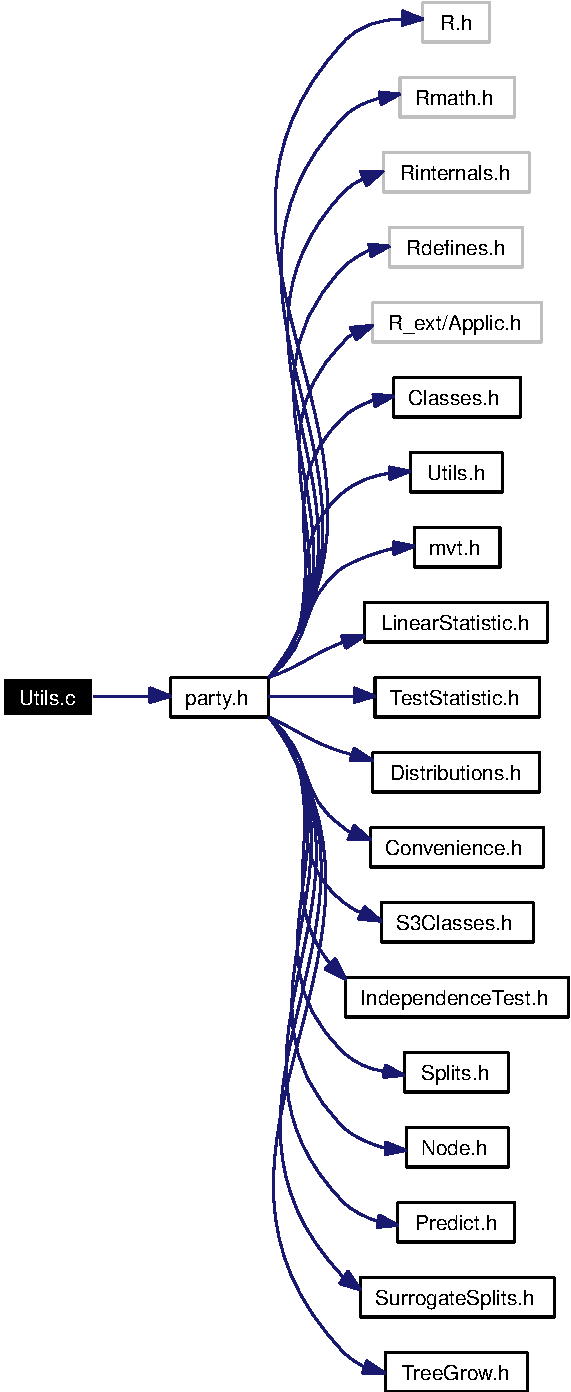
\includegraphics[width=154pt]{Utils_8c__incl}
\end{center}
\end{figure}
\subsection*{Functions}
\begin{CompactItemize}
\item 
void \hyperlink{Utils_8c_a0}{C\_\-kronecker} (const double $\ast$A, const int m, const int n, const double $\ast$B, const int r, const int s, double $\ast$ans)
\item 
SEXP \hyperlink{Utils_8c_a1}{R\_\-kronecker} (SEXP A, SEXP B)
\item 
SEXP \hyperlink{Utils_8c_a2}{CR\_\-svd} (SEXP x, SEXP svdmem)
\item 
void \hyperlink{Utils_8c_a3}{C\_\-MPinv} (SEXP x, double tol, SEXP svdmem, SEXP ans)
\item 
SEXP \hyperlink{Utils_8c_a4}{R\_\-MPinv} (SEXP x, SEXP tol, SEXP svdmem)
\item 
double \hyperlink{Utils_8c_a5}{C\_\-max} (const double $\ast$x, const int n)
\item 
SEXP \hyperlink{Utils_8c_a6}{R\_\-max} (SEXP x)
\item 
void \hyperlink{Utils_8c_a7}{C\_\-abs} (double $\ast$x, int n)
\item 
SEXP \hyperlink{Utils_8c_a8}{R\_\-abs} (SEXP x)
\item 
void \hyperlink{Utils_8c_a9}{C\_\-matprod} (double $\ast$x, int nrx, int ncx, double $\ast$y, int nry, int ncy, double $\ast$z)
\item 
SEXP \hyperlink{Utils_8c_a10}{R\_\-matprod} (SEXP x, SEXP y)
\item 
void \hyperlink{Utils_8c_a11}{C\_\-matprod\-T} (double $\ast$x, int nrx, int ncx, double $\ast$y, int nry, int ncy, double $\ast$z)
\item 
SEXP \hyperlink{Utils_8c_a12}{R\_\-matprod\-T} (SEXP x, SEXP y)
\item 
void \hyperlink{Utils_8c_a13}{C\_\-Sample\-No\-Replace} (int $\ast$x, int m, int k, int $\ast$ans)
\item 
SEXP \hyperlink{Utils_8c_a14}{R\_\-permute} (SEXP m)
\item 
SEXP \hyperlink{Utils_8c_a15}{R\_\-rsubset} (SEXP m, SEXP k)
\item 
int \hyperlink{Utils_8c_a16}{i\_\-in\_\-set} (int i, int $\ast$iset, int p)
\item 
int \hyperlink{Utils_8c_a17}{C\_\-i\_\-in\_\-set} (int i, SEXP set)
\item 
int \hyperlink{Utils_8c_a18}{nrow} (SEXP x)
\item 
int \hyperlink{Utils_8c_a19}{ncol} (SEXP x)
\item 
int \hyperlink{Utils_8c_a20}{C\_\-whichmax} (double $\ast$pvalue, double $\ast$teststat, int ninputs)
\item 
SEXP \hyperlink{Utils_8c_a21}{R\_\-whichmax} (SEXP x, SEXP y)
\item 
SEXP \hyperlink{Utils_8c_a22}{R\_\-listplus} (SEXP a, SEXP b, SEXP which)
\item 
SEXP \hyperlink{Utils_8c_a23}{R\_\-modify\_\-response} (SEXP x, SEXP vf)
\end{CompactItemize}


\subsection{Detailed Description}
Some commonly needed utility functions.

\begin{Desc}
\item[Author:]\begin{Desc}
\item[Author]hothorn \end{Desc}
\end{Desc}
\begin{Desc}
\item[Date:]\begin{Desc}
\item[Date]2006-04-05 16:24:23 +0200 (Wed, 05 Apr 2006) \end{Desc}
\end{Desc}


Definition in file \hyperlink{Utils_8c-source}{Utils.c}.

\subsection{Function Documentation}
\hypertarget{Utils_8c_a7}{
\index{Utils.c@{Utils.c}!C_abs@{C\_\-abs}}
\index{C_abs@{C\_\-abs}!Utils.c@{Utils.c}}
\subsubsection[C\_\-abs]{\setlength{\rightskip}{0pt plus 5cm}void C\_\-abs (double $\ast$ {\em x}, int {\em n})}}
\label{Utils_8c_a7}


absolute value \begin{Desc}
\item[Parameters:]
\begin{description}
\item[{\em x}]numeric vector \item[{\em n}]length(x)\end{description}
\end{Desc}


Definition at line 259 of file Utils.c.

Referenced by C\_\-absstandardize(), and R\_\-abs().\hypertarget{Utils_8c_a17}{
\index{Utils.c@{Utils.c}!C_i_in_set@{C\_\-i\_\-in\_\-set}}
\index{C_i_in_set@{C\_\-i\_\-in\_\-set}!Utils.c@{Utils.c}}
\subsubsection[C\_\-i\_\-in\_\-set]{\setlength{\rightskip}{0pt plus 5cm}int C\_\-i\_\-in\_\-set (int {\em i}, SEXP {\em set})}}
\label{Utils_8c_a17}




Definition at line 473 of file Utils.c.

References i\_\-in\_\-set().

Referenced by C\_\-get\_\-node().

Here is the call graph for this function:\begin{figure}[H]
\begin{center}
\leavevmode
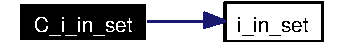
\includegraphics[width=94pt]{Utils_8c_a17_cgraph}
\end{center}
\end{figure}
\hypertarget{Utils_8c_a0}{
\index{Utils.c@{Utils.c}!C_kronecker@{C\_\-kronecker}}
\index{C_kronecker@{C\_\-kronecker}!Utils.c@{Utils.c}}
\subsubsection[C\_\-kronecker]{\setlength{\rightskip}{0pt plus 5cm}void C\_\-kronecker (const double $\ast$ {\em A}, const int {\em m}, const int {\em n}, const double $\ast$ {\em B}, const int {\em r}, const int {\em s}, double $\ast$ {\em ans})}}
\label{Utils_8c_a0}


Computes the Kronecker product of two matrices\par
 \begin{Desc}
\item[Parameters:]
\begin{description}
\item[{\em A}]matrix \item[{\em m}]nrow(A) \item[{\em n}]ncol(A) \item[{\em B}]matrix \item[{\em r}]nrow(B) \item[{\em s}]ncol(B) \item[{\em ans}]return value; a pointer to a REALSXP-vector of length (mr x ns)\end{description}
\end{Desc}


Definition at line 23 of file Utils.c.

Referenced by C\_\-Expect\-Covar\-Linear\-Statistic(), and R\_\-kronecker().\hypertarget{Utils_8c_a9}{
\index{Utils.c@{Utils.c}!C_matprod@{C\_\-matprod}}
\index{C_matprod@{C\_\-matprod}!Utils.c@{Utils.c}}
\subsubsection[C\_\-matprod]{\setlength{\rightskip}{0pt plus 5cm}void C\_\-matprod (double $\ast$ {\em x}, int {\em nrx}, int {\em ncx}, double $\ast$ {\em y}, int {\em nry}, int {\em ncy}, double $\ast$ {\em z})}}
\label{Utils_8c_a9}


matrix product x $\ast$\% y \begin{Desc}
\item[Parameters:]
\begin{description}
\item[{\em x}]a matrix \item[{\em nrx}]number of rows of x \item[{\em ncx}]number of cols of x \item[{\em y}]a matrix \item[{\em nry}]number of rows of y \item[{\em ncy}]number of cols of y \item[{\em z}]a matrix of dimension nrx x ncy\end{description}
\end{Desc}


Definition at line 297 of file Utils.c.

Referenced by C\_\-MLinear\-Statistic(), R\_\-matprod(), and R\_\-predict\-RF2().\hypertarget{Utils_8c_a11}{
\index{Utils.c@{Utils.c}!C_matprodT@{C\_\-matprodT}}
\index{C_matprodT@{C\_\-matprodT}!Utils.c@{Utils.c}}
\subsubsection[C\_\-matprodT]{\setlength{\rightskip}{0pt plus 5cm}void C\_\-matprod\-T (double $\ast$ {\em x}, int {\em nrx}, int {\em ncx}, double $\ast$ {\em y}, int {\em nry}, int {\em ncy}, double $\ast$ {\em z})}}
\label{Utils_8c_a11}


matrix product x $\ast$\% t(y) \begin{Desc}
\item[Parameters:]
\begin{description}
\item[{\em x}]a matrix \item[{\em nrx}]number of rows of x \item[{\em ncx}]number of cols of x \item[{\em y}]a matrix \item[{\em nry}]number of rows of y \item[{\em ncy}]number of cols of y \item[{\em z}]a matrix of dimension nrx x ncy\end{description}
\end{Desc}


Definition at line 349 of file Utils.c.

Referenced by C\_\-MLinear\-Statistic(), and R\_\-matprod\-T().\hypertarget{Utils_8c_a5}{
\index{Utils.c@{Utils.c}!C_max@{C\_\-max}}
\index{C_max@{C\_\-max}!Utils.c@{Utils.c}}
\subsubsection[C\_\-max]{\setlength{\rightskip}{0pt plus 5cm}double C\_\-max (const double $\ast$ {\em x}, const int {\em n})}}
\label{Utils_8c_a5}


the maximum of a double vector \begin{Desc}
\item[Parameters:]
\begin{description}
\item[{\em x}]vector \item[{\em n}]its length\end{description}
\end{Desc}


Definition at line 222 of file Utils.c.

Referenced by C\_\-maxabs\-Test\-Statistic(), C\_\-Monte\-Carlo(), C\_\-Node(), and R\_\-max().\hypertarget{Utils_8c_a3}{
\index{Utils.c@{Utils.c}!C_MPinv@{C\_\-MPinv}}
\index{C_MPinv@{C\_\-MPinv}!Utils.c@{Utils.c}}
\subsubsection[C\_\-MPinv]{\setlength{\rightskip}{0pt plus 5cm}void C\_\-MPinv (SEXP {\em x}, double {\em tol}, SEXP {\em svdmem}, SEXP {\em ans})}}
\label{Utils_8c_a3}


Moore-Penrose inverse of a matrix \begin{Desc}
\item[Parameters:]
\begin{description}
\item[{\em x}]matrix \item[{\em tol}]a tolerance bound \item[{\em svdmem}]an object of class `svd\_\-mem' \item[{\em ans}]return value; an object of class `Expect\-Covar\-MPinv'\end{description}
\end{Desc}


Definition at line 128 of file Utils.c.

References CR\_\-svd(), PL2\_\-MPinv\-Sym, PL2\_\-rank\-Sym, and PL2\_\-svd\-Sym.

Referenced by C\_\-Lin\-Stat\-Exp\-Cov\-MPinv(), and R\_\-MPinv().

Here is the call graph for this function:\begin{figure}[H]
\begin{center}
\leavevmode
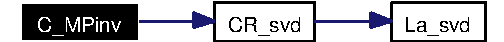
\includegraphics[width=134pt]{Utils_8c_a3_cgraph}
\end{center}
\end{figure}
\hypertarget{Utils_8c_a13}{
\index{Utils.c@{Utils.c}!C_SampleNoReplace@{C\_\-SampleNoReplace}}
\index{C_SampleNoReplace@{C\_\-SampleNoReplace}!Utils.c@{Utils.c}}
\subsubsection[C\_\-SampleNoReplace]{\setlength{\rightskip}{0pt plus 5cm}void C\_\-Sample\-No\-Replace (int $\ast$ {\em x}, int {\em m}, int {\em k}, int $\ast$ {\em ans})}}
\label{Utils_8c_a13}


compute a permutation of a (random subset of) 0:(m-1) \begin{Desc}
\item[Parameters:]
\begin{description}
\item[{\em x}]an integer vector of length m \item[{\em m}]integer \item[{\em k}]integer \item[{\em ans}]an integer vector of length k\end{description}
\end{Desc}


Definition at line 397 of file Utils.c.

Referenced by C\_\-Global\-Test(), C\_\-Monte\-Carlo(), R\_\-Ensemble(), R\_\-permute(), and R\_\-rsubset().\hypertarget{Utils_8c_a20}{
\index{Utils.c@{Utils.c}!C_whichmax@{C\_\-whichmax}}
\index{C_whichmax@{C\_\-whichmax}!Utils.c@{Utils.c}}
\subsubsection[C\_\-whichmax]{\setlength{\rightskip}{0pt plus 5cm}int C\_\-whichmax (double $\ast$ {\em pvalue}, double $\ast$ {\em teststat}, int {\em ninputs})}}
\label{Utils_8c_a20}




Definition at line 492 of file Utils.c.

Referenced by C\_\-Node(), and R\_\-whichmax().\hypertarget{Utils_8c_a2}{
\index{Utils.c@{Utils.c}!CR_svd@{CR\_\-svd}}
\index{CR_svd@{CR\_\-svd}!Utils.c@{Utils.c}}
\subsubsection[CR\_\-svd]{\setlength{\rightskip}{0pt plus 5cm}SEXP CR\_\-svd (SEXP {\em x}, SEXP {\em svdmem})}}
\label{Utils_8c_a2}


C- and R-interface to La\_\-svd (R/src/main/lapack.c) \begin{Desc}
\item[Parameters:]
\begin{description}
\item[{\em x}]matrix \item[{\em svdmem}]an object of class `svd\_\-mem'\end{description}
\end{Desc}


Definition at line 97 of file Utils.c.

References La\_\-svd(), PL2\_\-jobu\-Sym, PL2\_\-jobv\-Sym, PL2\_\-method\-Sym, PL2\_\-p\-Sym, PL2\_\-s\-Sym, PL2\_\-svd\-Sym, PL2\_\-u\-Sym, and PL2\_\-v\-Sym.

Referenced by C\_\-MPinv().

Here is the call graph for this function:\begin{figure}[H]
\begin{center}
\leavevmode
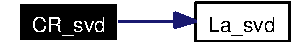
\includegraphics[width=87pt]{Utils_8c_a2_cgraph}
\end{center}
\end{figure}
\hypertarget{Utils_8c_a16}{
\index{Utils.c@{Utils.c}!i_in_set@{i\_\-in\_\-set}}
\index{i_in_set@{i\_\-in\_\-set}!Utils.c@{Utils.c}}
\subsubsection[i\_\-in\_\-set]{\setlength{\rightskip}{0pt plus 5cm}int i\_\-in\_\-set (int {\em i}, int $\ast$ {\em iset}, int {\em p})}}
\label{Utils_8c_a16}


determine if i is element of the integer vector set \begin{Desc}
\item[Parameters:]
\begin{description}
\item[{\em i}]an integer \item[{\em iset}]a pointer to an integer vector \item[{\em p}]length(iset)\end{description}
\end{Desc}


Definition at line 458 of file Utils.c.

Referenced by C\_\-i\_\-in\_\-set(), and C\_\-splitnode().\hypertarget{Utils_8c_a19}{
\index{Utils.c@{Utils.c}!ncol@{ncol}}
\index{ncol@{ncol}!Utils.c@{Utils.c}}
\subsubsection[ncol]{\setlength{\rightskip}{0pt plus 5cm}int ncol (SEXP {\em x})}}
\label{Utils_8c_a19}




Definition at line 484 of file Utils.c.

Referenced by C\_\-Global\-Test(), C\_\-Independence\-Test(), C\_\-MLinear\-Statistic(), C\_\-Monte\-Carlo(), C\_\-Node(), C\_\-splitnode(), R\_\-Ensemble(), R\_\-Expect\-Covar\-Influence(), R\_\-Expect\-Covar\-Linear\-Statistic(), R\_\-Linear\-Statistic(), R\_\-matprod(), R\_\-matprod\-T(), R\_\-MPinv(), R\_\-Node(), R\_\-Permuted\-Linear\-Statistic(), R\_\-predict\-RF2(), R\_\-split(), R\_\-splitcategorical(), and R\_\-Tree\-Grow().\hypertarget{Utils_8c_a18}{
\index{Utils.c@{Utils.c}!nrow@{nrow}}
\index{nrow@{nrow}!Utils.c@{Utils.c}}
\subsubsection[nrow]{\setlength{\rightskip}{0pt plus 5cm}int nrow (SEXP {\em x})}}
\label{Utils_8c_a18}




Definition at line 480 of file Utils.c.

Referenced by C\_\-Global\-Test(), C\_\-Independence\-Test(), C\_\-MLinear\-Statistic(), R\_\-Expect\-Covar\-Influence(), R\_\-Expect\-Covar\-Linear\-Statistic(), R\_\-Linear\-Statistic(), R\_\-matprod(), R\_\-matprod\-T(), R\_\-maxabs\-Conditional\-Pvalue(), R\_\-MPinv(), R\_\-Permuted\-Linear\-Statistic(), R\_\-predict\-RF2(), R\_\-split(), and R\_\-splitcategorical().\hypertarget{Utils_8c_a8}{
\index{Utils.c@{Utils.c}!R_abs@{R\_\-abs}}
\index{R_abs@{R\_\-abs}!Utils.c@{Utils.c}}
\subsubsection[R\_\-abs]{\setlength{\rightskip}{0pt plus 5cm}SEXP R\_\-abs (SEXP {\em x})}}
\label{Utils_8c_a8}


R-interface to C\_\-abs \begin{Desc}
\item[Parameters:]
\begin{description}
\item[{\em x}]numeric vector\end{description}
\end{Desc}


Definition at line 271 of file Utils.c.

References C\_\-abs().

Here is the call graph for this function:\begin{figure}[H]
\begin{center}
\leavevmode

\includegraphics[width=82pt]{Utils_8c_a8_cgraph}
\end{center}
\end{figure}
\hypertarget{Utils_8c_a1}{
\index{Utils.c@{Utils.c}!R_kronecker@{R\_\-kronecker}}
\index{R_kronecker@{R\_\-kronecker}!Utils.c@{Utils.c}}
\subsubsection[R\_\-kronecker]{\setlength{\rightskip}{0pt plus 5cm}SEXP R\_\-kronecker (SEXP {\em A}, SEXP {\em B})}}
\label{Utils_8c_a1}


R-interface to C\_\-kronecker \begin{Desc}
\item[Parameters:]
\begin{description}
\item[{\em A}]matrix \item[{\em B}]matrix\end{description}
\end{Desc}


Definition at line 52 of file Utils.c.

References C\_\-kronecker().

Here is the call graph for this function:\begin{figure}[H]
\begin{center}
\leavevmode

\includegraphics[width=110pt]{Utils_8c_a1_cgraph}
\end{center}
\end{figure}
\hypertarget{Utils_8c_a22}{
\index{Utils.c@{Utils.c}!R_listplus@{R\_\-listplus}}
\index{R_listplus@{R\_\-listplus}!Utils.c@{Utils.c}}
\subsubsection[R\_\-listplus]{\setlength{\rightskip}{0pt plus 5cm}SEXP R\_\-listplus (SEXP {\em a}, SEXP {\em b}, SEXP {\em which})}}
\label{Utils_8c_a22}




Definition at line 527 of file Utils.c.\hypertarget{Utils_8c_a10}{
\index{Utils.c@{Utils.c}!R_matprod@{R\_\-matprod}}
\index{R_matprod@{R\_\-matprod}!Utils.c@{Utils.c}}
\subsubsection[R\_\-matprod]{\setlength{\rightskip}{0pt plus 5cm}SEXP R\_\-matprod (SEXP {\em x}, SEXP {\em y})}}
\label{Utils_8c_a10}


R-interface to C\_\-matprod \begin{Desc}
\item[Parameters:]
\begin{description}
\item[{\em x}]a matrix \item[{\em y}]a matrix\end{description}
\end{Desc}


Definition at line 318 of file Utils.c.

References C\_\-matprod(), ncol(), and nrow().

Here is the call graph for this function:\begin{figure}[H]
\begin{center}
\leavevmode
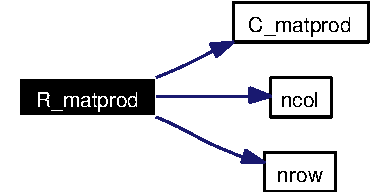
\includegraphics[width=102pt]{Utils_8c_a10_cgraph}
\end{center}
\end{figure}
\hypertarget{Utils_8c_a12}{
\index{Utils.c@{Utils.c}!R_matprodT@{R\_\-matprodT}}
\index{R_matprodT@{R\_\-matprodT}!Utils.c@{Utils.c}}
\subsubsection[R\_\-matprodT]{\setlength{\rightskip}{0pt plus 5cm}SEXP R\_\-matprod\-T (SEXP {\em x}, SEXP {\em y})}}
\label{Utils_8c_a12}


R-interface to C\_\-matprod\-T \begin{Desc}
\item[Parameters:]
\begin{description}
\item[{\em x}]a matrix \item[{\em y}]a matrix\end{description}
\end{Desc}


Definition at line 370 of file Utils.c.

References C\_\-matprod\-T(), ncol(), and nrow().

Here is the call graph for this function:\begin{figure}[H]
\begin{center}
\leavevmode
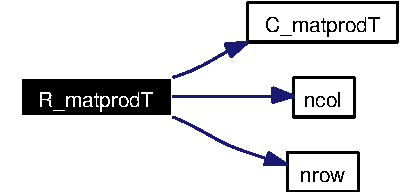
\includegraphics[width=108pt]{Utils_8c_a12_cgraph}
\end{center}
\end{figure}
\hypertarget{Utils_8c_a6}{
\index{Utils.c@{Utils.c}!R_max@{R\_\-max}}
\index{R_max@{R\_\-max}!Utils.c@{Utils.c}}
\subsubsection[R\_\-max]{\setlength{\rightskip}{0pt plus 5cm}SEXP R\_\-max (SEXP {\em x})}}
\label{Utils_8c_a6}


R-interface to C\_\-max \begin{Desc}
\item[Parameters:]
\begin{description}
\item[{\em x}]numeric vector\end{description}
\end{Desc}


Definition at line 238 of file Utils.c.

References C\_\-max().

Here is the call graph for this function:\begin{figure}[H]
\begin{center}
\leavevmode
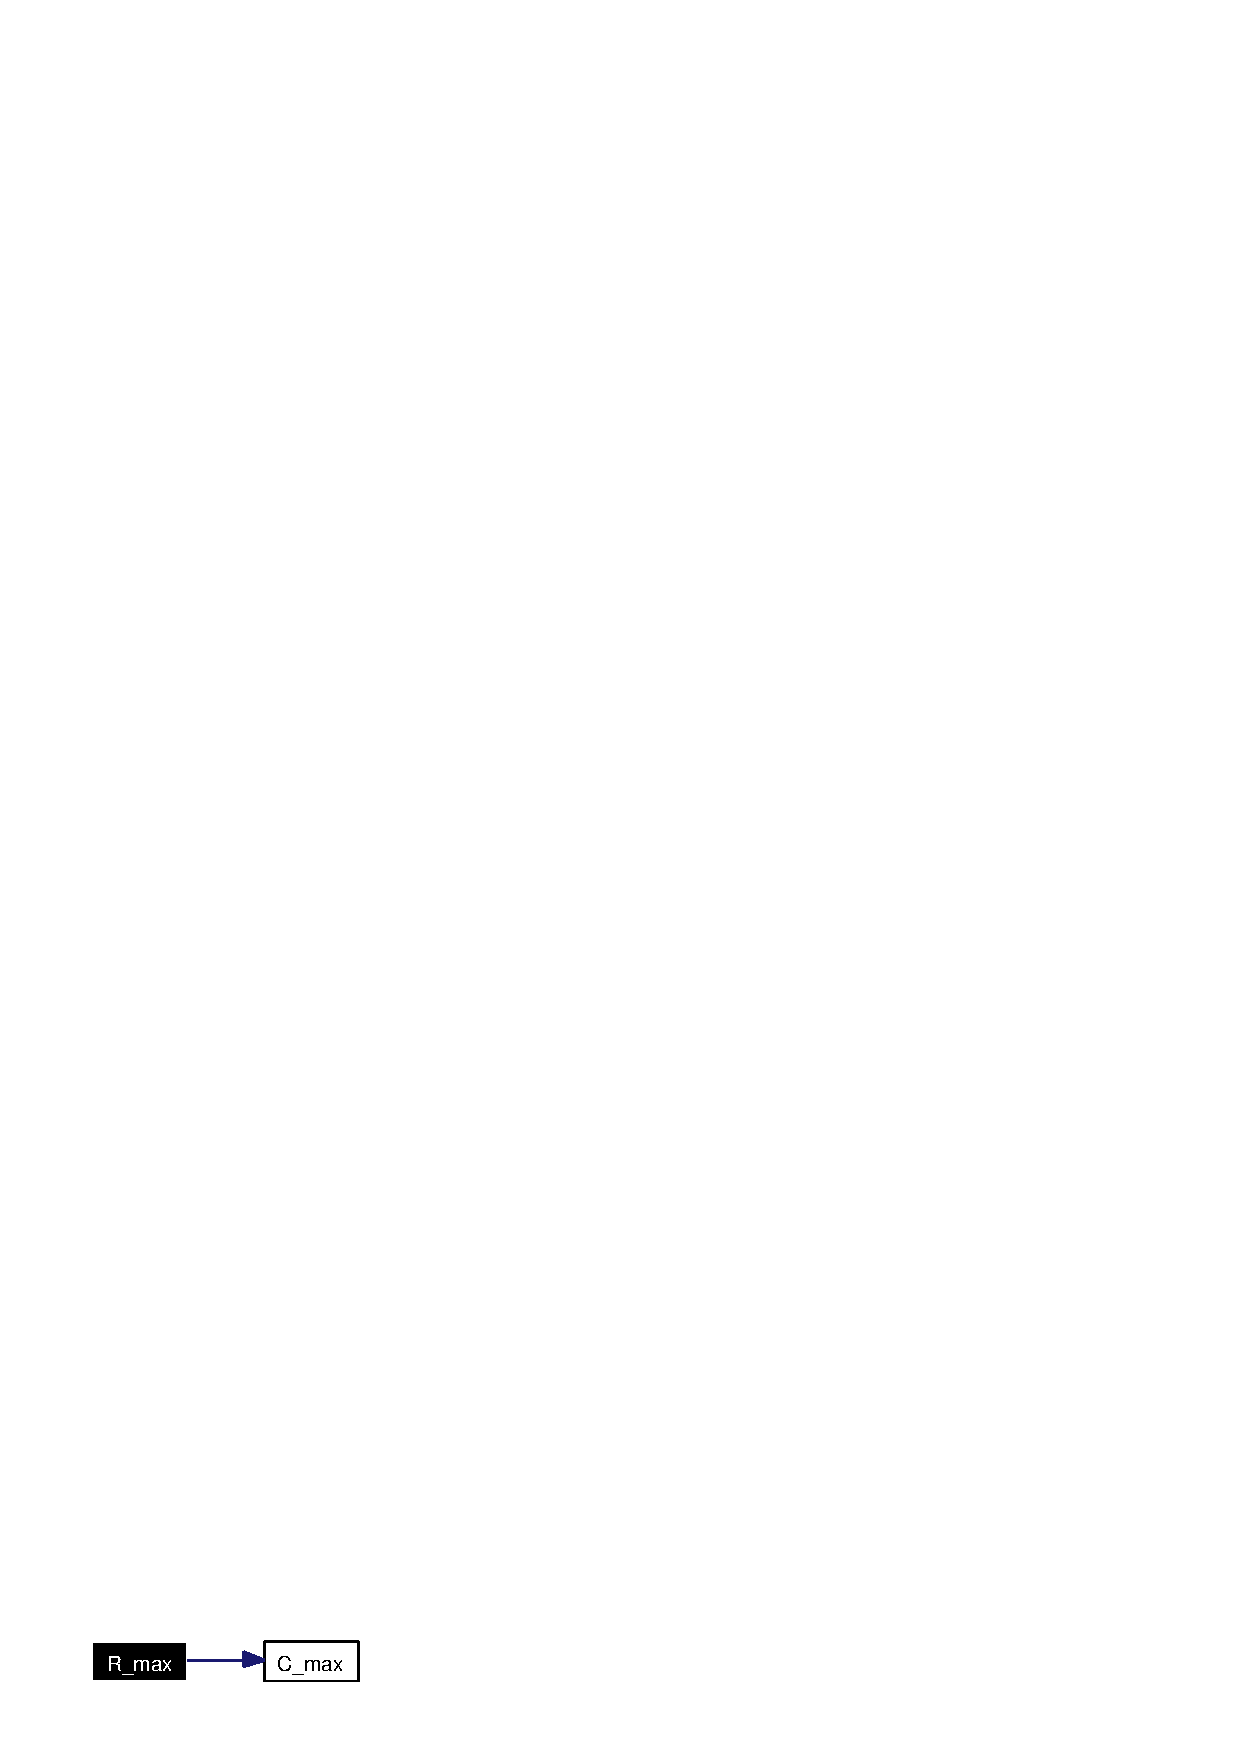
\includegraphics[width=84pt]{Utils_8c_a6_cgraph}
\end{center}
\end{figure}
\hypertarget{Utils_8c_a23}{
\index{Utils.c@{Utils.c}!R_modify_response@{R\_\-modify\_\-response}}
\index{R_modify_response@{R\_\-modify\_\-response}!Utils.c@{Utils.c}}
\subsubsection[R\_\-modify\_\-response]{\setlength{\rightskip}{0pt plus 5cm}SEXP R\_\-modify\_\-response (SEXP {\em x}, SEXP {\em vf})}}
\label{Utils_8c_a23}




Definition at line 559 of file Utils.c.

References get\_\-jointtransf(), get\_\-transformation(), and get\_\-variable().

Here is the call graph for this function:\begin{figure}[H]
\begin{center}
\leavevmode
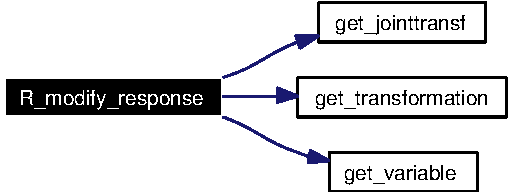
\includegraphics[width=139pt]{Utils_8c_a23_cgraph}
\end{center}
\end{figure}
\hypertarget{Utils_8c_a4}{
\index{Utils.c@{Utils.c}!R_MPinv@{R\_\-MPinv}}
\index{R_MPinv@{R\_\-MPinv}!Utils.c@{Utils.c}}
\subsubsection[R\_\-MPinv]{\setlength{\rightskip}{0pt plus 5cm}SEXP R\_\-MPinv (SEXP {\em x}, SEXP {\em tol}, SEXP {\em svdmem})}}
\label{Utils_8c_a4}


R-interface to C\_\-MPinv \begin{Desc}
\item[Parameters:]
\begin{description}
\item[{\em x}]matrix \item[{\em tol}]a tolerance bound \item[{\em svdmem}]an object of class `svd\_\-mem'\end{description}
\end{Desc}


Definition at line 187 of file Utils.c.

References C\_\-MPinv(), ncol(), nrow(), PL2\_\-MPinv\-Sym, PL2\_\-p\-Sym, and PL2\_\-rank\-Sym.

Here is the call graph for this function:\begin{figure}[H]
\begin{center}
\leavevmode
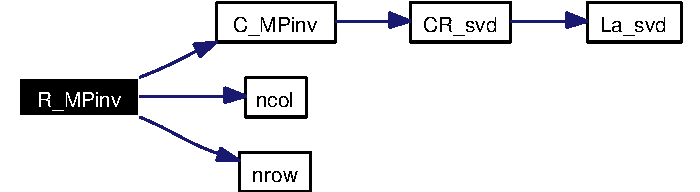
\includegraphics[width=181pt]{Utils_8c_a4_cgraph}
\end{center}
\end{figure}
\hypertarget{Utils_8c_a14}{
\index{Utils.c@{Utils.c}!R_permute@{R\_\-permute}}
\index{R_permute@{R\_\-permute}!Utils.c@{Utils.c}}
\subsubsection[R\_\-permute]{\setlength{\rightskip}{0pt plus 5cm}SEXP R\_\-permute (SEXP {\em m})}}
\label{Utils_8c_a14}


R-interface to C\_\-Sample\-No\-Replace: the permutation case \begin{Desc}
\item[Parameters:]
\begin{description}
\item[{\em m}]integer\end{description}
\end{Desc}


Definition at line 416 of file Utils.c.

References C\_\-Sample\-No\-Replace().

Here is the call graph for this function:\begin{figure}[H]
\begin{center}
\leavevmode

\includegraphics[width=125pt]{Utils_8c_a14_cgraph}
\end{center}
\end{figure}
\hypertarget{Utils_8c_a15}{
\index{Utils.c@{Utils.c}!R_rsubset@{R\_\-rsubset}}
\index{R_rsubset@{R\_\-rsubset}!Utils.c@{Utils.c}}
\subsubsection[R\_\-rsubset]{\setlength{\rightskip}{0pt plus 5cm}SEXP R\_\-rsubset (SEXP {\em m}, SEXP {\em k})}}
\label{Utils_8c_a15}


R-interface to C\_\-Sample\-No\-Replace: the subset case \begin{Desc}
\item[Parameters:]
\begin{description}
\item[{\em m}]integer \item[{\em k}]integer\end{description}
\end{Desc}


Definition at line 436 of file Utils.c.

References C\_\-Sample\-No\-Replace().

Here is the call graph for this function:\begin{figure}[H]
\begin{center}
\leavevmode

\includegraphics[width=123pt]{Utils_8c_a15_cgraph}
\end{center}
\end{figure}
\hypertarget{Utils_8c_a21}{
\index{Utils.c@{Utils.c}!R_whichmax@{R\_\-whichmax}}
\index{R_whichmax@{R\_\-whichmax}!Utils.c@{Utils.c}}
\subsubsection[R\_\-whichmax]{\setlength{\rightskip}{0pt plus 5cm}SEXP R\_\-whichmax (SEXP {\em x}, SEXP {\em y})}}
\label{Utils_8c_a21}




Definition at line 517 of file Utils.c.

References C\_\-whichmax().

Here is the call graph for this function:\begin{figure}[H]
\begin{center}
\leavevmode
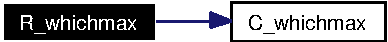
\includegraphics[width=110pt]{Utils_8c_a21_cgraph}
\end{center}
\end{figure}
